\begin{figure}
\begin{subfigure}{0.475\textwidth}
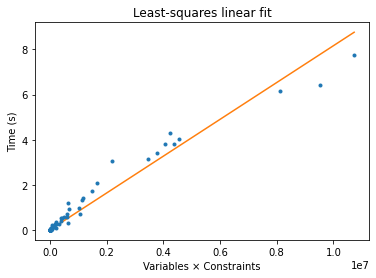
\includegraphics[width=0.9\textwidth]{images/least-squares-solve.png}
\caption{\solve execution time vs. $\norm{V}\norm{C}$ \\ (blue dots), linear model (orange line)}
\label{fig:stats:linregress-solve}
\end{subfigure}
\hfill
\begin{subfigure}{0.475\textwidth}
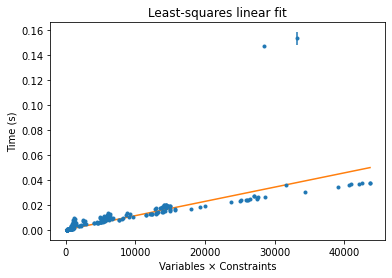
\includegraphics[width=0.9\textwidth]{images/least-squares-RecCheck.png}
\caption{\RecCheck execution time vs. $\norm{V}\norm{C}$ \\ (blue dots), linear model (orange line)}
\label{fig:stats:linregress-reccheck}
\end{subfigure}
\\[3ex]
\begin{subfigure}{0.475\textwidth}
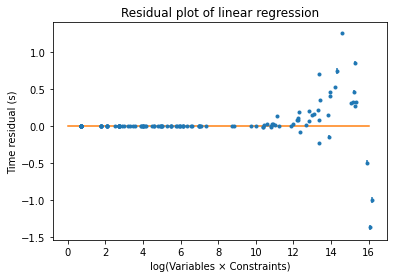
\includegraphics[width=0.9\textwidth]{images/residuals-solve.png}
\caption{\solve model residuals plot (log scale)}
\label{fig:stats:residuals-solve}
\end{subfigure}
\hfill
\begin{subfigure}{0.475\textwidth}
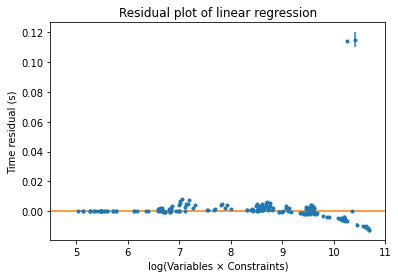
\includegraphics[width=0.9\textwidth]{images/residuals-RecCheck.png}
\caption{\RecCheck model residuals plot (log scale)}
\label{fig:stats:residuals-reccheck}
\end{subfigure}
\\[3ex]
\begin{subfigure}{0.475\textwidth}
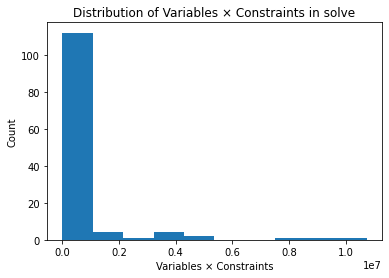
\includegraphics[width=0.9\textwidth]{images/distribution-solve.png}
\caption{$\norm{V}\norm{C}$ distribution in \solve, 10 bins}
\label{fig:stats:distr-solve}
\end{subfigure}
\hfill
\begin{subfigure}{0.475\textwidth}
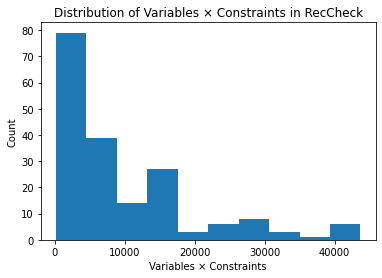
\includegraphics[width=0.9\textwidth]{images/distribution-RecCheck.png}
\caption{$\norm{V}\norm{C}$ distribution in \RecCheck, 10 bins}
\label{fig:stats:distr-reccheck}
\end{subfigure}
\\[2ex]
\caption{Execution vs. $\norm{V}\norm{C}$, linear model residuals, and $\norm{V}\norm{C}$ distribution plots for \solve and \RecCheck}
\label{fig:stats}
\end{figure}

\begin{figure}
\begin{minted}{coq}
Unset Guard Checking.
Set Sized Typing.
Time Definition nats1  := (nat, nat, nat, nat, nat, nat, nat, nat).
Time Definition nats2  := (nats1, nats1, nats1, nats1).
Time Definition nats3  := (nats2, nats2, nats2, nats2).
Time Definition nats4  := (nats3, nats3, nats3, nats3).
Time Definition nats5  := (nats4, nats4, nats4, nats4).
Time Definition nats6  := (nats5, nats5, nats5, nats5).
\end{minted}
\caption{Coq definitions with an explosion in size variables and elapsed time}
\label{fig:nats}
\end{figure}